% ! Tex program = xelatex
\documentclass{article}
% 中文
% \usepackage[UTF8]{ctex}

%! Tex program = xelatex
% \documentclass{article}
%中文
%\usepackage[UTF8]{ctex}
%数学公式
\usepackage{amsmath,amssymb}
%\usepackage{ntheorem}
% \usepackage[framemethod=TikZ]{mdframed}
\usepackage{amsthm}
%边界
\usepackage[letterpaper,top=2cm,bottom=3cm,left=2cm,right=2cm,marginparwidth=1.75cm]{geometry}%table package
%Table
\usepackage{multirow,booktabs}
\usepackage{makecell}
%字体颜色
\usepackage{color}
% \usepackage[dvipsnames]{xcolor}  % 更全的色系
%代码
\usepackage[OT1]{fontenc}
% MATLAB 代码风格
%\usepackage[framed,numbered,autolinebreaks,useliterate]{/Users/anye_zhenhaoyu/Desktop/Latex/mcode}
\usepackage{listings}
\usepackage{algorithm}
\usepackage{algorithmic}
\usepackage{pythonhighlight} % Python
%插图
\usepackage{graphicx}
%改变item格式
\usepackage{enumerate}
%物理
\usepackage{physics}
%extra arrows
\usepackage{extarrows}
% caption(居中指令)
%\usepackage[justification=centering]{caption}
\usepackage{caption}
% htpb
\usepackage{stfloats}
% pdf 拼接
\usepackage{pdfpages}
% 超链接url
\usepackage{url}
\usepackage{tikz}
\usepackage{pgfplots}
\pgfplotsset{compat=newest}
\usepackage[colorlinks=true, allcolors=red]{hyperref}
\usepackage{setspace}
\usepackage{bbm}

% --------------definations-------------- %
\def\*#1{\boldsymbol{#1}}
\def\+#1{\mathcal{#1}} 
\def\-#1{\mathrm{#1}}
\def\rm#1{\mathrm{#1}}
\def\=#1{\mathbb{#1}}
% Domains
\def\RR{\mathbb{R}}
\def\EE{\mathbb{E}}
\def\CC{\mathbb{C}}
\def\NN{\mathbb{N}}
\def\ZZ{\mathbb{Z}}
% Newcommand
\newcommand{\inner}[2]{\langle #1,#2\rangle} 
\newcommand{\numP}{\#\mathbf{P}} 
\renewcommand{\P}{\mathbf{P}}
\newcommand{\Var}[2][]{\mathbf{Var}_{#1}\left[#2\right]}
\newcommand{\E}[2][]{\mathbf{E}_{#1}\left[#2\right]}
\renewcommand{\emptyset}{\varnothing}
\newcommand{\ol}{\overline}
\newcommand{\argmin}{\mathop{\arg\min}}
\newcommand{\argmax}{\mathop{\arg\max}}
\renewcommand{\abs}[1]{\qty|#1|}
\newcommand{\defeq}{\triangleq} % triangle over =
\def\deq{\xlongequal{def}} % 'def' over =
\def\LHS{\text{LHS}}
\def\RHS{\text{RHS}}
\def\angbr#1{\langle#1\rangle} % <x>
\def\set#1{\qty{#1}}

\def\Esolve{\textcolor{blue}{Solve: }}
\def\Eproof{\textcolor{blue}{Proof: }}
\def\case#1{\textcolor{blue}{Case \uppercase\expandafter{\romannumeral#1}: }}

% \newmdtheoremenv{lemma}{Lemma}
% \newmdtheoremenv{theorem}{\textcolor{red}{Theorem}}
% \newmdtheoremenv{defi}{\textcolor{blue}{Definition}}
\newtheorem{lemma}{Lemma}
\newtheorem{thm}{Theorem}
\newtheorem{defi}{Definition}
\newtheorem{prp}{Proposition}
\newtheorem{remark}{Remark}
\newenvironment{md}{\begin{mdframed}}{\end{mdframed}}

\graphicspath{{figures/}}

% \begin{document}
% \title{<++>}
\author{Haoyu Zhen}
% \maketitle
\setlength{\parindent}{0pt}
\setstretch{1.2}
% \end{document}

\usepackage{fancyhdr}
\pagestyle{fancy}
% \fancypagestyle{mainFancy}{
%     \fancyhf{}
%     \renewcommand\headrulewidth{.5pt}       % 页眉横线
%     \renewcommand\footrulewidth{0pt}
%     \fancyhead[OC]{\fzkai{\leftmark}}       % 页眉章标题
%     \fancyhead[EC]{\fzkai{\@title}}         % 页眉文章题目
% 	\lhead{\fzkai{author}}
%     \fancyhead[OR,EL]{\thepage}                 % 页眉编号
%     \fancyfoot[r]{\thumb} % 将拇指放到没有被使用的页眉或页脚处
% }
\fancyhf{}
\fancyfoot[C]{\thepage}
\fancyhead[R]{\slshape{AI2615 Algorithm Design and Analysis}}
\fancyhead[L]{\slshape{Haoyu Zhen}}


\graphicspath{{figures/}}

\begin{document}
% \tableofcontents
\title{Written assginment 1}
\maketitle
\section*{Question 1}
\subsection*{(a)}

$\displaystyle \norm{x-y}^2=\int_{0}^{T} \qty[x(t)-c]^2 \,\dd t=\int_{0}^{T} x^2(t) \,\dd t - 2c \int_{0}^{T} x(t) \,\dd t + c^2T$.
To minimize the distance between $x$ and $y$,
\[
	c=\frac{1}{T}\int_{0}^{T} x(t) \,\dd t
	.\]

\subsection*{(b)}
Let $e(t)=\flatfrac{1}{\sqrt{T}}$ if  $t\in[0,T)$ otherwise  $e(t)=0$. Then  $\forall f \in V$, we have $f=f(0)e(t)$, which means that  $V=\text{span}(e)$. And $\displaystyle \int_{0}^{T} \qty(\flatfrac{1}{\sqrt{T}})^2 \,\dd t=1\Longrightarrow\angbr{e,e}=1$.

Then
\[
	y(t)=\qty[{\int_{0}^{T} x(t)e(t) \,\dd t}]e(t) = \qty[\frac{1}{\sqrt{T}}\int_{0}^{T} x(t) \,\dd t] e(t)
	.\]
Thus $\displaystyle y(t)=\frac{1}{T}\int_{0}^{T} x(t) \,\dd t$ if  $t\in[0,T)$ otherwise  $e(t)=0$.

\subsection*{(c)}
Obviously the result in (a) coincides with that in (b). I prefer the second method because we no not need to optimize any objective function.


\section*{Question 2}
\subsection*{(a)}
\begin{prp}
	$\forall f \in V$, \[f(t)=f(-1)\varphi_{-1}(t)+f(0)\varphi_0(t)+f(1)\varphi_1(t).\]
\end{prp}
\begin{proof}
	$\forall t\in[0,1]$, $f(t)=[f(1)-f(0)]t+f(0)=f(0)\varphi_0(t)+f(1)\varphi_1(t)$.

	And $\forall t\in[-1,0)$, $f(t)=[f(0)-f(-1)]t+f(0)=f(-1)\varphi_{-1}(t)+f(0)\varphi_0(t)$.
\end{proof}
Thus $f=f(-1)\varphi_{-1}+f(0)\varphi_0+f(1)\varphi_1$.


\subsection*{(b)}
Obviously, $\varphi_1$ and $\varphi_{-1}$ are orthogonal.

\subsection*{(c)}
$\displaystyle
	\int_{-1}^{1} \varphi_{-1}(t)\varphi_0(t) \,\dd t
	=
	\int_{-1}^{1} \varphi_{1}(t)\varphi_0(t) \,\dd t
	=
	\frac{1}{6}
$ and
$\displaystyle
	\int_{-1}^{1} \varphi_{-1}^2(t) \,\dd t
	=
	\int_{-1}^{1} \varphi_{1}^2(t) \,\dd t
	=\frac{1}{3}
$. Then
\[
	\hat{\varphi}_0=\varphi_0-\frac{1}{2}\varphi_{-1}-\frac{1}{2}\varphi_1=
	\begin{cases}
		1.5t+1, & \mbox{if }t\in[-1,0] \\
		1-1.5t, & \mbox{if }t\in(0,1]  \\
		0,      & \mbox{otherwise}
	\end{cases}
	.\]

\begin{figure}[H]
	\centering
	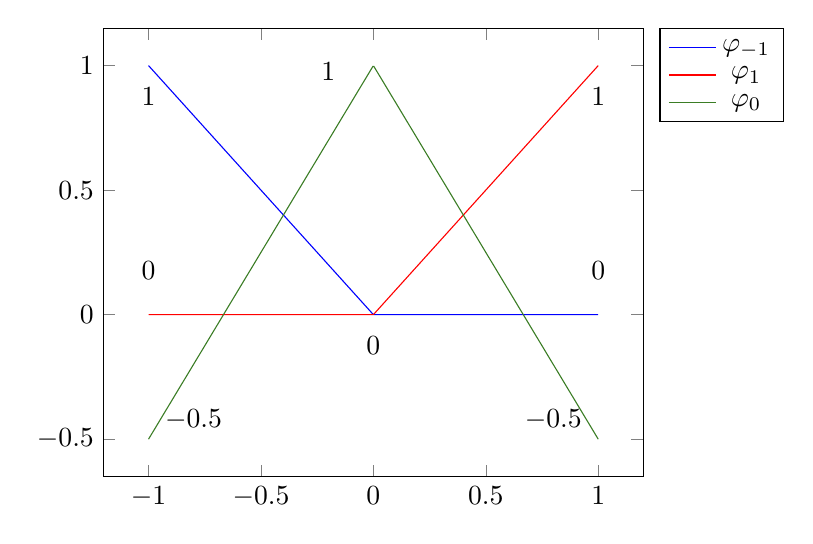
\begin{tikzpicture}
		\begin{axis}[samples=500,domain= -1 : 1 ,restrict y to domain = -1 : 1, legend pos=outer north east]
			\addplot[blue] plot ({\x},{max(min(abs(\x/2)-\x/2, 1), -1)});
			\addlegendentry{$\varphi_{-1}$}
			\addplot[red] plot ({\x},{max(min(abs(\x/2)+\x/2, 1), -1)});
			\addlegendentry{$\varphi_{1}$}
			\addplot[OliveGreen] plot ({\x},{max(min(-abs(1.5*\x)+1, pi), -pi)});
			\addlegendentry{$\varphi_{0}$}
			\coordinate[label=$0$] (0) at (0,-0.2);
			\coordinate[label=$1$] (0) at (1,0.8);
			\coordinate[label=$1$] (0) at (-1,0.8);
			\coordinate[label=$1$] (0) at (-0.2,0.9);
			\coordinate[label=$0$] (0) at (-1,0.1);
			\coordinate[label=$0$] (0) at (1,0.1);
			\coordinate[label=$-0.5$] (0) at (-0.8,-0.5);
			\coordinate[label=$-0.5$] (0) at (0.8,-0.5);
		\end{axis}
	\end{tikzpicture}
\end{figure}


\subsection*{(d)}
What we want to solve is:
\[
	f_0=\argmin_f \int_{-1}^{1} \qty[g(t)-f(t)]^2 \,\dd t
	=
	\argmin_f \qty[\int_{-1}^{1} f^2(t) \,\dd t - 2 \int_{-1}^{1} g(t)f(t) \,\dd t]
	.\]
Assume that $f = a\varphi_{-1}+b\hat{\varphi}_0+c\varphi_1$.

Then $\displaystyle \int_{-1}^{1} f^2(t) \,\dd t = \frac{1}{3}a^2+\frac{1}{2}b^2+\frac{1}{3}c^2$ and $\displaystyle \int_{-1}^{1} g(t)f(t) \,\dd t=\frac{1}{2}a+\frac{7}{12}b+\frac{2}{9}c$.

By the fact that
\[
	\argmin_{[a,b,c]}\qty(\frac{1}{3}a^2+\frac{1}{2}b^2+\frac{1}{3}c^2-a-\frac{7}{6}b-\frac{4}{9}c)=\qty[\frac{3}{2},\,\frac{7}{6},\,\frac{2}{3}]
	,\]
	$\displaystyle f=\frac{3}{2}\varphi_{-1}+\frac{7}{6}\hat{\varphi_0}+\frac{2}{3}\varphi_1$.

% \begin{figure}[H]
%     \centering
%     \begin{tikzpicture}
%         \begin{axis}[samples=500,domain= -1 : 1 ,restrict y to domain = -1 : 1]
%         \addplot[blue] plot ({\x},{max(min(-abs(2/3*\x)-5/12*\x+7/6, 1), -1)});
%         \end{axis}
%     \end{tikzpicture}
% \end{figure}

\begin{figure}[H]
	\centering
	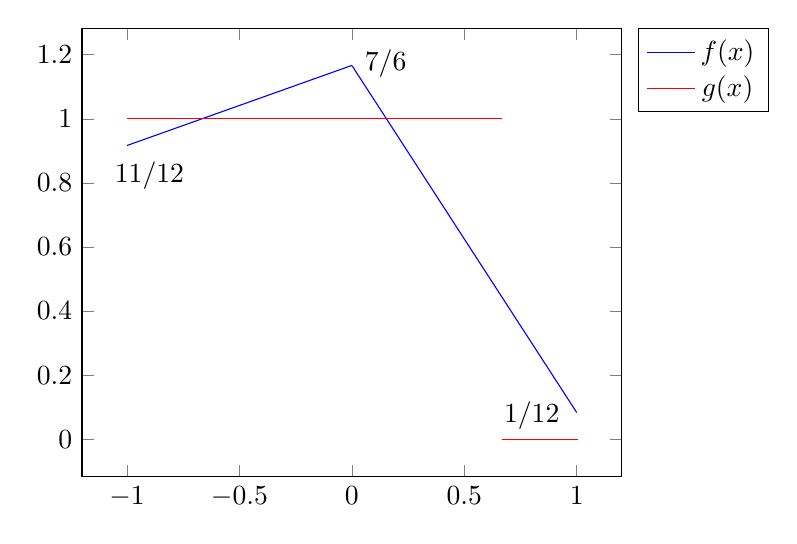
\begin{tikzpicture}
		\begin{axis}[samples=500,domain= -1 : 1 ,restrict y to domain = -1 : 1.2, legend pos=outer north east]
			\addplot[blue] plot ({\x},{max(min(-abs(2/3*\x)-5/12*\x+7/6, 1.2), -1)});
			\addplot[domain=-1:2/3,color=red] plot ({\x},{max(min(1, 1.2), -1)});
			\addplot[domain=2/3:1,color=red] plot ({\x},{max(min(0, 1.2), -1)});
			\legend{$f(x)$, $g(x)$}
			\coordinate[label=$\flatfrac{7}{6}$] (0) at (0.15,1.1);
			\coordinate[label=$\flatfrac{1}{12}$] (0) at (0.8,0);
			\coordinate[label=$\flatfrac{11}{12}$] (0) at (-0.9,0.75);
		\end{axis}
	\end{tikzpicture}
\end{figure}


\end{document}
